\chapter{Supervised and Unsupervised learning}
We limit our focus to supervised and unsupervised learning if not specified otherwise, reinforcement learning will be treated later on.
\todo{Solve problem with bold greek letters}
\section{More formal introduction into the idea of Machine Learning}
\subsection{Problem set-up and recipe}
\label{subsec:recipeML}
Problems in ML typically involve inference about complex systems where we do not know the exact form of the mathematical model that describes the system. It is therefore not uncommon to have multiple candidate models that need to be compared.
\subsubsection{Ingredients}
Many problems in ML and data science start with the same ingredients. The first ingredient is the dataset $\mD=(\mX,\mathbf{y})$ where $\mX$ is a matrix of independent variables and $\mathbf{y}$ is a vector of dependent variables. The second is the model $f(\mx;\mt)$, which is a function $f:\mx \rightarrow y$ of the \emph{parameters} $\mt$. That is, $f$ is a function used to predict an output from a vector of input variables. 
\marginpar{Using polynomial models (i.e. polynomials of different order) in polynomial regressions, we can think of each term in the polynomial as a ’feature’ (i.e. a,b are features for $f_1(x)=a x^2+bx$) in our model, then increasing the order of the polynomial we fit increases the number of features.}
\begin{mybox}{Model class}
	To make predictions, we will consider a family of functions $f_{\alpha}(x,\mt_\alpha)$ that depend on some parameters $\mt_\alpha$. These functions represent the \emph{model class} that we are using to model the data and make predictions. Note that we choose the model class without knowing the function $f(x)$. The $f_\alpha(x;\mt_\alpha)$ encode the \emph{features} we choose to represent the data. Different models (e.g. $\alpha=1,2,3$) can contain different number of parameters, then the models have different \emph{model complexity}.
\end{mybox}
The final ingredient is the \emph{cost function} $\mC(\my,f(\mX;\mt))$ that allow us to judge how well the model performs on the observations $\my$. The model is fit by finding the value of $\mt$ that minimizes the cost function. For example, one commonly used cost function is the squared error. Minimizing the squared error cost function is known as the method of least squares, and is typically appropriate for experiments with Gaussian measurement errors.
\subsubsection{Recipe}
\begin{enumerate} 
\item The \emph{first step} in the analysis is to \emph{randomly} divide the dataset $\mD$ into two mutually exclusive groups $\mD_{train}$ and $\mD_{test}$ called the training and test sets. The fact that this must be the first step should be heavily emphasized - performing some analysis (such as using the data to select important variables) before partitioning the data is a common pitfall that can lead to incorrect conclusions. Typically, the majority of the data are partitioned into the training set (e.g. $90\%$) with the remainder going into the test set. 
\begin{mybox}{Cross evaluation}
	Therefore, to learn the parameters $\mt_\alpha$, we will train our models on a \emph{training dataset} and then test the effectiveness of the model on a \textbf{different} dataset, the \emph{test dataset}.
\end{mybox}
\item The model is fit by minimizing the cost function using only the data in the training set $\hat{\mt}= \arg \min_{θ}\{\mC(\my_{train}, f(\mX_{train};\mt) )\}$.
\item Finally, the performance of the model is evaluated by computing the cost function using the test set $\mC(\my_{test},f(\mX_{test};\hat{\mt}))$. 
\end{enumerate}
\subsection{Performance evaluation}
\label{subsec:performanceeval}
\subsubsection{Ingredients for performance evaluation}
\begin{mybox}{Measure for evaluating performance}
	The value of the cost function for the best fit model on the training set is called the \emph{in-sample error}
	\be 
	\label{eq:errorInsample}
	E_{in}=\mC(\my_{train},f(\mX_{train};\mt))
	\ee 
	and the value of the cost function on the test set is called the \emph{out-of-sample error}
	\be 
	\label{eq:errorOutsample}
	E_{out}= \mC(\my_{test},f(\mX_{test};\mt)).
	\ee 
	One of the most important observations we can make is that \textbf{the out-of-sample error is almost always greater than the in-sample error}
	\be 
	\label{eq:errorComparison}
	E_{out} \geq E_{in}.
	\ee 
	Comparison of candidate models is usually done by using $E_{out}$. The model that minimizes this out-of-sample error is chosen as the best model (i.e. model selection).
\end{mybox}
Note that once we select the best model on the basis of its performance on $E_{out}$, the real-world performance of the winning model should be expected to be slightly worse because the test data was now used in the fitting procedure.\\
Splitting the data into mutually exclusive training and test sets provides an unbiased estimate for the predictive performance of the model - this is known as \emph{cross-validation}.
\begin{mybox}{Pitfalls for performance evaluation}
	It may be at first surprising that the model that has the lowest out-of-sample error $E_{out}$ usually \emph{does not} have the lowest in-sample Error $E_{in}$. Therefore, if our goal is to obtain a model that is useful for prediction, we may not want to choose the model that provides the best explanation for the current observations. At first glance, the observation that the model providing the best explanation for the current dataset probably will not provide the best explanation for future datasets is very counter-intuitive. \\
Moreover, the discrepancy between $E_{in}$ and $E_{ou}$ becomes more and more important, as the complexity of our data, and the models we use to make predictions, grows. As the number of parameters in the model increases, we are forced to work in high-dimensional spaces. The ’curse of dimensionality’ ensures that many phenomena that are absent or rare in low-dimensional spaces become generic.
\end{mybox}
A comment on the difference between the in-and out-of-sample errors:\\
There is a fundamental difference between minimizing the in-sample error and minimizing the out-of-sample error. The underlying reason for this is that the training data may not be representative of the full data distribution. From a Bayesian point of view, as David MacKay likes to repeat: \emph{We can't make predictions without making assumptions}. Thus, it is sensible to introduce priors that reflect the fact that we are likely to be undersampled (especially in high dimensions).
\subsubsection{Another mathematical measure for performance evaluation}
\begin{mybox}{$R^2$ coefficient of determination}
	 The model performance (in-sample and out-of-sample) can be evaluated using the so-called \emph{coefficient of determination}, which is given by:
		\be
	\label{eq:errorR2}
	R^2=1-\frac{\sum_{i=1}^n \abs{y^{true}_i - y^{pred}_i}^2}{\sum_{i=1}^n \abs{y^{true}_i- \frac{1}{n} \sum_{i=1}^n y^{pred}_i}^2}.
	\ee 
Optimal performance is $R^2=1$. but it can also be negative. A constant model that always predicts the expected value of $y, ⟨y^{true}⟩,$ disregarding the input features, would get a $R^2$ score of $0$.
\end{mybox}
















\subsubsection{How to effectively do the performance evaluation}
It turns out that for complicated models studied in ML, predicting and fitting are very different things.\\
	Models that give the best fit to existing data do not necessarily make the best predictions even for simple tasks. At small sample sizes, noise can create fluctuations in the data that look like genuine patterns. Simple models (like a linear function) cannot represent complicated patterns in the data, so they are forced to ignore the fluctuations and to focus on the larger trends. 
\begin{mybox}{Overfitting}
	\label{subsubsec:overfitting}
Complex models with many parameters can capture both the global trends and noise-generated patters at the same time. IN this case, the model can be tricked into thinking that the noise encodes real information. This problem is called \emph{overfitting} and leads to a steep drop-off in predictive performance.\\
We can guard against overfitting in two ways:
\begin{enumerate}
	\item We can use less expensive models with fewer parameters, or
	\item we can collect more data so that the likelihood that the noise appears patterned decreases.
\end{enumerate}
The relative degree of overfitting: This information is contained in the difference in accuracy of our model on the training  and test datasets.
\end{mybox}
\begin{mybox}{Bias-Variance tradeoff}
	\label{subsubsec:biasvariancetradeoff}
	The \emph{bias-variance} tradeoff is used in our countermeasures against overfitting. What is it ?\\When the amount of training data is limited, one can often get better predictive power performance by using a less expressive model rather than the more complex model. The simpler model has more ’bias’ but is less dependent on the particular realization of the training dataset, i.e. less ’variance’. Therefore, even though the correct model is guaranteed to have better predictive performance for an infinite amount of training data (less bias), the training errors stemming from finite-size sampling (variance) can cause simpler models to outperform the more complex model when sampling is limited.
\end{mybox}
The bias-variance tradeoff is one of the key concepts in ML and therefore discussed quantitatively in more detail in \ref{subsubsec:biasvariancetradeoff} and qualitatively in \ref{subsubsec:biasvarianceMathematical}.\\
These two concepts are now discussed in more detail, for that we introduce another quantity and then look explicitly at the components of our theory causing problems for different complexity regimes.
\begin{mybox}{Bias}
	The bias represents the best our model could do if we had an infinite amount of training data to beat down sampling noise. The bias is a property of the kind of functions, or model class, we are using to approximate $f(x)$. In general, the more complex the model class we use, the smaller the bias. However, we do not generally have an infinite amount of data. For this reason, to get best predictive power it is better to minimize the out-of-sample error, $E_{out}$, rather than the bias. 
\end{mybox}\footnote{This stems from the the law of large number. This is a theorem that describes the result of performing the same experiment a large number of times. According to the law, the average of the results obtained from a large number of trials should be close to the expected value and will tend to become closer to the expected value as more trials are performed}
How can we get a better idea of what is the true object to minimize to get bets results ? \\
The Bias-Variance tradeoff is implicitly encoded in the in-and out-of-sample errors. We will therefore draw from statistical learning theory in the following to get a better understanding of what it is we ought to be doing to achieve best practices.\\
\subsubsection{Where do the insights about how to do best practices come from ?}
The out-of-sample error will decrease with the number of data points. As the number of data points gets large, the sampling noise decreases and the training data set becomes more representative of the true distribution from which the data is drawn. For this reason, in the infinite data limit, the in-sample and out-of-sample error must approach the same value, which is called the ’bias’ of our model.

\begin{figure}[h!]
	\centering
	\includegraphics[width=0.7\linewidth]{gfx/IMG_20200303_180633}
	\caption{}
	\label{fig:errorbehaviour}
\end{figure}
Compare the behaviour of both errors with increasing number of data points, left graph of \ref{fig:errorbehaviour}, and the out-of-sample error with increasing model complexity, right graph of \ref{fig:errorbehaviour}. As for the left graph, we can look at the difference between the generalization ($\abs{E_{in}-E_{out}}$) and training error ($E_{in}$), the big curly bracket. It measures how well our in-sample error reflects the out-of-sample error, and measures how much worse we would do on a new data set compared to our training data. For this reason, the difference between these error is precisely the quantity that measures the difference between fitting and predicting. \emph{Models with a large difference between the in-sample and out-of-sample errors are said to \textbf{overfit} the data}. 
\begin{mybox}{}
	One of the lessons of statistical learning theory is that it is not enough to simply minimize the training error, because the out-of-sample error can still be large.
\end{mybox}
Considering the right graph, model  complexity is, in many cases, related to the number of parameters we are using to approximate the true function $f(x)$. If we consider a training dataset of a fixed size, $E_{out}$ will be a non-monotonic function of the model complexity, and is generally minimized for models with \emph{intermediate} complexity. The underlying reason for this is that, even though using a more complicated model always reduces the bias, at some point the model becomes too complex for the amount of training data and the generalization error becomes large due to high variance.
\begin{mybox}{}
Thus, to minimize $E_{out}$ and maximize our predictive power, it may be more suitable to use a more biased model with small variance than a less-biased model with large variance. This is is, again, the \emph{bias-variance} tradeoff we introduced above.
\end{mybox} 
Another way to understand this tradeoff is the following. Due to sampling noise from having finite size data sets, the learned models will differ for each choice of training sets. In general, more complex models need a larger amount of training data. For this reason, the fluctuations in the learned models (variance) will be much larger for the more complex model than the simpler model. However, if we consider the asymptotic performance as we increase the size of the training set (the bias), it is clear that the complex model will eventually perform better than the simpler model. Thus, depending on the amount of training data, it may \textbf{be more favourable to use a less comples, high-bias model to make predictions}.
























\section{Statistics}
Statistical modelling revolves around estimation or prediction.
\subsection{Difference between estimation and prediction}
Note first and foremost that techniques in ML tend to be more focused on prediction rather than estimation, which means that we will mostly treat prediction problems in this compendium. This is for example because an artificially intelligent agent needs to be able to recognize objects in its surroundings and predict the behaviour of its environment in order to make informed choices.\\
\subsubsection{Contrasting the two}
Estimation and prediction problems can be cast into a common conceptual framework. In both cases, we choose some observable quantity $\mx$ of the system we are studying (e.g. an interference pattern) that is related to some parameters $\mt$ (e.g. the speed of light) of a model $p(\mx|\mt)$ that describes the probability of observing $\mx$ given $\mt$.\\
Now we perform an experiment to obtain a dataset $\mX$ and use these data to fit the model. Typically,  ’fitting’ the model involves finding $\hat{\mt}$ that provides the best explanation for the data. IN the case when ’fitting’ refers to the method of least squares, the estimated parameters maximize the probability of observing the data (i.e., $\hat{\mt}=\arg \max_{\mt}\{p(\mX|\mt) \}$).\\
\begin{mybox}{Estimation vs Prediction}
	\emph{Estimation problems} are concerned with the accuracy of $\hat{\mt}$, whereas \emph{prediction problems} are concerned with the ability of the model to predict new observations (i.e., the accuracy of $p(\mx|\hat{\mt})$. Although the goals of estimation and prediction are related, they often lead to different approaches.
\end{mybox}


\subsection{Mathematical motivation to presented key ideas}
We begin with an unknown function
$y = f (x)$ and fix a \emph{hypothesis set} $\mH$ consisting of all functions we are willing to consider, defined also on the domain of $f$ . This set may be uncountably infinite (e.g. if
there are real-valued parameters to fit). The choice of
which functions to include in $\mH$ usually depends on our
intuition about the problem of interest. The function
$f (x)$ produces a set of pairs $(x_i , y_i ), i = 1 . . . N$ , which
serve as the observable data. Our goal is to select a function from the hypothesis set $h \in \mH$ that approximates
$f (x)$ as best as possible, namely, we would like to find
$h \in \mH$ such that $h \approx f$ in some strict mathematical
sense which we specify below. 
\begin{mybox}{}
If this is possible, we say
that we \emph{learned} $f (x)$. 
\end{mybox}
But if the function $f (x)$ can, in
principle, take any value on \emph{unobserved inputs}, how is it
possible to learn in any meaningful sense ?\\
The answer is that learning is possible in the restricted
sense that the fitted model will probably perform approximately as well on new data as it did on the training data.
How can we evaluate the performance of our model then ?\\
As discussed in \ref{subsec:performanceeval}, once an appropriate error function $E$ is chosen for the
problem under consideration (e.g. sum of squared errors
in linear regression), we can define the in-and out-of-sample error to then minimize the out-of-sample error, with the variance-bias tradeoff in mind, to achieve robust predictions.
\subsubsection{Bias-Variance Decomposition for one Classifier}
\label{subsubsec:biasvarianceMathematicaloneClassifier}
Here we give a mathematical motivation to the bias-variance tradeoff discussed in \ref{subsubsec:biasvariancetradeoff}.\\
Consider a
dataset $\mD = (\mx, \mathbf{y})$ consisting of the $N$ pairs of independent and dependent variables. Let us assume that the
true data is generated from a noisy model
\be 
y = f (x) + \epsilon
\ee 
where $\epsilon$ is normally distributed with mean zero and standard deviation $\sigma_\epsilon$, i.e. the ’noise’.
Assume that we have a statistical procedure (e.g. least-
squares regression) for forming a predictor $f (\mx; \hat{\mathbf{θ}})$ that
gives the prediction of our model for a new data point $\mx$.
This estimator is chosen by minimizing a cost function
which we take to be the squared error
\be 
\label{eq:statCostFct}
\mC(\mathbf{y}, f(\mx; \mathbf{θ})) = \sum_i (y_i - f(x_i; \mathbf{θ}))^2.
\ee 
Therefore, the estimates for the parameters
\be 
\hat{\mathbf{θ}} =\arg \min_{θ} \mC(\mathbf{y}, f(\mx;\mathbf{θ}) )
\ee 
are a function of the dataset, $\mD$. We would obtain a
different error $\mC( \mathbf{y}_j , f (\mx_j ; \hat{\mathbf{θ}}_{\mD_j}))$ for each dataset $\mD_j =
(\mathbf{y}_j , \mx_j )$ in a universe of possible datasets obtained by
drawing $N$ samples from the true data distribution. We
denote an expectation value over all of these datasets as
$\mathbb{E}_{\mD}$.


\begin{mybox}{Errors}
	Combining these expressions,
	we see that the expected \emph{out-of-sample error}
	\be 
	 E_{out} := \mathbb{E}_{\mD,\epsilon}[\mC(\mathbf{y}, f (\mx; \hat{\mathbf{θ}}_{\mD} ))],
	\ee 
	 can be decomposed as
	 \be 
	E_{out} = \text{Bias}^2 + \text{Var} + \text{Noise},
	\ee
	with
	\begin{align*}
	\text{Noise}&=\sum_i \sigma^2_\epsilon,\; \text{Var}=\sum_i \mathbb{E}_{\mD}[(f (\mx_i ; \hat{\mathbf{θ}}_{\mD} ) − \mathbb{E}_{\mD}[f (\mx_i ; \hat{\mathbf{{θ}}}_{\mD})])^2 ],\\
	\text{Bias}^2&=\sum_i (f (\mx_i ) − \mathbb{E}_{\mD}[f ((\mx_i ;\hat{(\mathbf{θ}}_{\mD} )])^2.
	\end{align*}
	The variance measures how much our estimator fluctuates due
	to finite-sample effects and the bias measures the deviation of the expectation value of
	our estimator (i.e. the asymptotic value of our estimator
	in the infinite data limit) from the true value.
\end{mybox}
This gives us a mathematical tradeoff of the concepts discussed in \ref{subsec:performanceeval} and in particular in \ref{fig:errorbehaviour}.
\begin{mybox}{Bias-variance trade-off}
	The bias-variance tradeoff summarizes the fundamental tension in machine learning, particularly supervised
	learning, between the complexity of a model and the
	amount of training data needed to train it. Since data
	is often limited, in practice it is often useful to use a
	less-complex model with higher bias – a model whose
	asymptotic performance is worse than another model –
	because it is easier to train and less sensitive to sampling
	noise arising from having a finite-sized training dataset
	(smaller variance).
\end{mybox}
\subsubsection{Bias-Variance Decomposition for Ensembles}
\label{subsubsec:biasvarianceMathematicalEnsemble}
We will discuss the bias-variance tradeoff in the context of continuous predictions such as regression \ref{sec:linearRegression}. However, many of the intuitions and ideas discussed here also carry over to classification tasks, cf. \ref{sec:logisticRegression}. Consider a data set consisting of data $\mX_{\mL}=\{(y_j,\mx_j),j=1\dots n \}$ as above. Assume that we have a statistical procedure (e.g. OLS \ref{eq:lregOLS})) for forming a predictor $\hat{g}_{\mL}(\mx)$ that gives the prediction of our model for a new data point $\mx$ given that we trained the model using a dataset $\mL$. We will now, however, consider an ensemble of estimators $\{\hat{g}_{\mL}(\mx_i)\}$. Given a dataset $\mX_{\mL}$ and hyper-parameters $\mt$ that parametrize members of our ensemble, we will consider a procedure that deterministically generates a model $\hat{g}_{\mL}(\mx_i,\mt)$ given $\mX_{\mL}$ and $\mt$. We assume that the $\mt$ includes some random parameters that introduce stochasticity into our ensemble (e.g. an initial condition for stochastic gradient descent or a random subset of features or data points used for training.) Concretely, with a given dataset $\mL$ one has a learning algorithm $\mA$ that generates a model $\mA(\mt,\mL)$ based on a deterministic procedure which introduced stochasticity through $\mt$ in its execution on dataset $\mL$. \\
We will be concerned with the expected prediction error of the \emph{aggregate ensemble predictor}
\be 
\label{eq:biasvarianceAggregateEnsemblePredictor}
\hat{g}^A_{\mL}(\mx_i,\{\mt\} ) = \frac{1}{M} \sum_{n=1}^M \hat{g}_{\mL}(\mx_i,\mt_m).
\ee 
For future reference, let us define the mean, variance and covariance (i.e. the connected correlation function in the language of physics), and the normalized correlation coefficient of a single randomized model $\hat{g}_{\mL}(\mx,\mt_m)$ as 
\begin{align}
	\label{eq:biasvarianceDefinitionsMoments}
	\mathbb{E}_{\mL,\mt_m}[\hat{g}_{\mL}(\mx,\mt_m)] &= \mu_{\mL,\mt_m}(\mx) \nonumber \\
	\mathbb{E}_{\mL,\mt_m}[\hat{g}_{\mL}(\mx,\mt_m)^2]- \mathbb{E}_{\mL,\mt_m}[\hat{g}_{\mL}(\mx,\mt)]^2 &= \sigma^2_{\mL,\mt_m}(\mx) \nonumber \\
	\mathbb{E}_{\mL,\mt_m}[\hat{g}_{\mL}(\mx,\mt_m) \hat{g}_{\mL}(\mx,\mt_{m^\prime})] -\mathbb{E}_{\mt}[\hat{g}_{\mL}(\mx,\mt_m) ]^2 &= C_{\mL,\mt_m,\mt_{m^\prime}} (\mx) \nonumber \\
	\rho(\mx) &= \frac{C_{\mL,\mt_m,\mt_{m^\prime}}(\mx) }{\sigma^2_{\mL,\mt}}.
\end{align}
Note that the expectation $\mathbb{E}_{\mL,\mt_m}[\cdot]$ is computed over the joint distribution of $\mL$ and $\mt_m$. Also by definition, we assume $m\neq m^\prime$.\\
Now, we can, as in \ref{subsubsec:biasvarianceMathematicaloneClassifier}, define the expected generalization (out-of-sample) error for the ensemble 
\begin{align}
\label{eq:biasvarianceGeneralizationErrorEnsemble}
\mathbb{E}_{\mL,\mt_m}[C(\mX,\hat{g}^A_{\mL}(\mx))] &= \mathbb{E}_{\mL,\epsilon,\mt} \left[ \sum_i (\my_i - \hat{g}^A_{\mL} (\mx_i,\{\mt\} ))^2\right]\nonumber \\
&= Bias^2(\mx_i) + Var(\mx_i)+ \sum_i \sigma^2_{\epsilon_i},
\end{align}
where one defines the bias of an aggregate predictor 
\be 
\label{eq:biasvarianceBiasEnesemble}
Bias^2(\mx) \equiv \left(f(\mx) - \mathbb{E}_{\mL,\mt}[\hat{g}^A_{\mL} (\mx,\{\mt\}) ]\right)^2
\ee 
and the variance as
\bse 
Var(\mx) = \\mathbb{E}_{\mL,\mt}\left[ (\hat{g}^A_{\mL}(\mx,\{\mt\}) - \mathbb{E}_{\mL,\mt}[\hat{g}^A_{\mL}(\mx,\{\mt\})])^2 \right]. 
\ese 
So far the calculation for ensembles is almost identical to that of a single estimator, compare \ref{subsubsec:biasvarianceMathematicaloneClassifier}.
\begin{mybox}{Crux of Bias-Variance for Ensembles}
	However, since the aggregate estimator is a sum of estimators, its variance implicitly depends on the correlations between the individual estimators in the ensemble. One finds
	\be 
	\label{eq:biasvarianceVarianceEnsembleCrux}
	Var(\mx) = \rho(\mx) \sigma^2_{\mL,\mt} + \frac{1-\rho(\mx)}{M} \sigma^2_{\mL,\mt}.
	\ee 
	This \ref{eq:biasvarianceVarianceEnsembleCrux} is the key to understanding the power of random ensembles. Notice that by using large ensembles ($M\rightarrow \infty$), we can significantly reduce the variance, and for completely random ensembles where the models are uncorrelated ($\rho(\mx)=0$), maximally suppresses the variance !\\
	Thus, reducing the aggregate predictor beats down fluctuations due to finite-sample effects. They key, as \ref{eq:biasvarianceVarianceEnsembleCrux} indicates, is to \textbf{decorrelate the models as much as possible while still using a very large ensemble.}
\end{mybox}
\begin{mybox}{What does this do to the bias ?}
One can be worried that this comes at the expense of a very large bias. This turns out not to be the case. When models in the ensemble are completely random, the bias of the aggregate predictor is just the expected bias of a single model 
\bse 
Bias^2(\mx) = (f(\mx) - \mu_{\mL,\mt})^2.
\ese 
\textbf{Thus, for a random ensemble one can always add more models without increasing the bias.}
\end{mybox}

Therefore, the correlation between models that constitute the ensemble is the key property here. It is important for two reasons. First, holding the ensemble size fixed, averaging the predictions of correlated models reduces the variance less than averaging uncorrelated models. Second, in some cases, correlations between models within an ensemble can result in an \emph{increase} in bias, offsetting any potential reduction in variance gained from ensemble averaging.\\
This will be discussed in the context of bagging \ref{subsec:ensemblesBagging}










\subsection{Mathematical set-up of every problem ever}
As described quantitatively in \ref{subsec:recipeML}, every problem in ML can be designed via a recipe which is presented now qualitatively.\\
\subsubsection{Set-up of the notation}
Suppose we are given a dataset with $n$ samples $\mD = \{(y_i,\mx^{(i)} )\}^n_{i=1}$, where $\mx^{(i)}$ is the $i$-th observation vector while $y_i$ is its corresponding (scalar) response. We assume that every sample has $p$ \emph{features}, namely,
\bse 
\mx^{(i)} \in \mR^p.
\ese  
Let $f$ be the true function/model that generated these samples via
\bse 
y_i  = f(\mx^{(i)}, \mw_{true}) + \epsilon_i,
\ese 
where $\mw_{true}\in \mR^p$ is a \emph{parameter} vector and $\epsilon_i$ is some i.i.d. white noise with zero mean and finite variance. Conventionally, we cast all samples in an $n\times p$ matrix, the \emph{design matrix}
\bse 
\mX \in \mR^{n\times p}
\ese 
with the rows 
\bse 
\mX_{i,:} = \mx^{(i)} \in \mR^p,\quad i =1,\dots,n
\ese 
being \emph{observations} and the columns
\bse 
\mX_{:,j} \in \mR^n,\quad j=1,\dots,p 
\ese 
being measured \emph{features}(i.e. feature predictors).\\
Bear in mind that this function $f$ is never known to us explicitly, though in practice we usually presume its functional form.
\begin{example}
	For example, in \emph{linear regression}, we assume
	\bse 
	y_i = f(\mx^{(i)};\mw_{true}) + \epsilon_i= \mw^T_{true} \mx^{(i)} + \epsilon_i
	\ese 
	for some unknown but fixed $\mw_{true}\in \mR^p$.
\end{example}










\subsubsection{Set-up of the problem}
We want to find a function $g$ with parameters $\mw$ fit to the data $\mD$ that can best approximate $f$. This is done when we have found a $\hat{\mw}$ such that $g(\mx;\hat{\mw})$ yields our best estimate of $f$. Now we can use this $g$ to make predictions about the response $y_0$ for a new data point $\mx_0$.\\
Therefore:\\
Fitting a given set of samples $(y_i,\mx_i)$ means relating the independent variables $\mx_i$ to their responses $y_i$. The next step is to assume some \emph{models} that might explain the measurements and measuring their performance, i.e. finding the function $g$ such that
\bse 
y_i = g(\mx_i;\mw).
\ese 
We call $g(\mx^{(i)},\mw)$ the \emph{predictor}. Recall that the optimal choice of predictor depends on, among many other things, the functions used to fit the data and the underlying noise level.
We then try to minimize the errors made in explaing the given set of measurements based on our model $g$ by tuning the parameters $\mw$. To do so, we need to first define the error function (formally called the  \emph{loss function}) that characterizes the deviation of our prediction form the actual response




\subsubsection{On statistical language}
As described above, a ML or statistics problem is defined via a optimization (minimization) problem of an error function, the solution to this is given by some estimator
\be 
\hat{\mw}_{Problem} = \arg \min_{\mw \in \mR^p} \mC(\mX, g(\mw,\my)).
\ee 
The bias (or bias function) of an estimator is the difference between this estimator's expected value and the true value of the parameter being estimated.


\subsection{Language of optimization problems}
\subsubsection{Convexity}
Recall that a set $C\subset\mR^n$ is called \emph{convex} if any  $x,y\in C$  and  $t\in [0,1]$,
\bse 
tx + (1-t) y \in C.
\ese 

In other words, every line segments joining  $x,y$  lies entirely in  $C$ .

A function $f:\mR^n \rightarrow \mR$ is called \emph{convex} if its domain $\text{dom}(f)$  is a convex set and for any  $x,y\in \text{dom}(f)$  and $ t\in[0,1]$ ,
\bse 
f(tx+(1-t)y) \leq t f(x) + (1-t) f(y).
\ese 

In other words, the function lies below the line segment joining $ f(x)$  and $ f(y)$ . This function  $f$  is called \emph{strictly convex} if this inequality holds strictly for  $x \neq y$  and  $t \in (0,1)$ .
\begin{mybox}{}
Why is convexity important? \\
\textbf{For convex functions, any local minimizer is a global minimizer}. Algorithmically, this means that in the minimization (optimization) procedure, as long as we're "going down the hill" and agree to stop when we can't go any further, then we've hit the global minimum. In addition to this, there's a menagerie of beautiful theory regarding convex duality and optimality, which gives us a way of understanding the solutions even before solving the problem itself.
\end{mybox}


\section{Overview of Bayesian Inference}
\label{sec:bayes}
Bayesian inference provides a set of principles and procedures for learning from data and for describing uncertainty.
\subsection{Language}
\begin{mybox}{Likelihood function}
	The \emph{likelihood function} 
	\be
	\label{eq:bayesLikelihoodFct}
	p(\mX|\mt)
	\ee 
	describes the probability of observing a dataset $\mX$ for a given value of the unknown parameters $\mt$. It is a function of the parameters $\mt$ with the data $\mX$ held fixed. Furthermore, it is determined by the model and the measurement noise.
\end{mybox}
\begin{mybox}{Prior distribution}
	The \emph{prior distribution} $p(\mt)$ describes any knowledge that we have about the parameters before we collect the data.
\end{mybox}
\begin{mybox}{Priors}
	\label{subsec:priors}
	There are two general classes of priors: 
	\begin{enumerate}
		\item The \emph{uninformative prior}:\\
		We choose this one if we do not have any specialized knowledge about $\mt$ before we look at the data. 
		\item The \emph{informative prior}:\\
		If we have prior knowledge, we choose an informative prior that accurately reflects the knowledge that we have about $\mt$. This one is commonly employed in ML:
	\end{enumerate}
	There is another not so important prior, the \emph{hierarchical prior}. This describes the process of choosing a hyperparameter by defining a prior distribution for it (via an uninformative prior) and then averaging the posterior distribution over all choices of the hyperparameter.
\end{mybox}
Using an informative prior tends to decrease the variance of the posterior distribution while, potentially, increasing its bias. It is beneficial if the decrease in variance is larger than the increase in bias. In high-dimensional problems, it is reasonable to assume that many of the parameters will not be strongly relevant. Therefore, many of the parameters of the model will be zero or close to zero. We can express this belief using two commonly used priors.
\begin{mybox}{Two informative priors commonly employed}
	The \emph{Gaussian prior} is used to express the assumption that many of the parameters will be small 
	\be 
	\label{eq:bayesGaussianprior}
	p(\mt|\lambda) = \prod_j \sqrt{\frac{\lambda}{2 \pi}} e^{- \lambda \theta^2_j},
	\ee
	where $\lambda$ is a \emph{hyperparameter}. The \emph{Laplace prior} is used to express the assumption that many of the parameters will be zero
	\be 
	\label{eq:bayesLaplacianprior}
	p(\mt|\lambda) = \prod_j \frac{\lambda}{2} e^{-\lambda \abs{\theta_j}}.
	\ee 
	The hyperparameter can either be chose via a hierarchical prior employing MCMC or  by simply finding a good value of $\lambda$ using an optimization procedure (see linear regression).
\end{mybox}
Indeed, a Gaussian prior is the \emph{conjugate prior} that gives a Gaussian posterior. For a given likelihood, conjugacy guarantees the preservation of prior distribution at the posterior level.
\begin{example}
	For example, for a Gaussian (Geometric) likelihood with a Gaussian (Beta) prior, the posterior distribution is still a Gaussian (Beta) distribution.
\end{example}
\begin{mybox}{hyperparameters}
	A \emph{hyperparameter} or \emph{nuisance variable} is a parameter whose value is set before the learning process begins. By contrast, the values of other \emph{parameters} are derived via training.
\end{mybox}

\subsubsection{Connecting statistics and bayesian framework}
To connect a statistical model to the Bayesian framework, we often write the model as
\be 
\label{eq:bayesianFreqConnectionModel}
p(y|\mx,\mt) = \mathcal{N}(y|\mu(\mx),\sigma^2(\mx)).
\ee 
In other words, our model is defined by a conditional probability that depends not only on data $\mx$ but on some model parameters $\mt$.
\begin{example}
	For example, if the mean is a linear function of $\mx$ given by $\mu = \mx^T \mw$, and the variance is fixed $\sigma^2(\mx) = \sigma^2$, then $\mt=(\mw,\sigma^2)$.
\end{example}











\subsection{Calculations}
\begin{mybox}{Bayes' rule}
	The \emph{posterior distribution} $p(\mt|\mX)$ describes our knowledge about the unknown parameter $\mt$ after observing the data $\mX$. It is given via Bayes' rule
	\be 
	\label{eq:bayesrule}
	p(\mt | \mX) = \frac{p(\mX|\mt) p(\mt) }{\int \md \mt^\prime p(\mX | \mt^\prime) p(\mt^\prime)}.
	\ee
\end{mybox}
The denominator is difficult in practice such that one normally uses Markov Chain Monte Carlo (MCMC) to draw random samples from $p(\mt|\mX)$.
\subsection{Estimation}
\subsubsection{Maximum Likelihood estimation}
In statistics, many problems rely on estimation of some parameters of interest.
\begin{example}
	For example, suppose we are given the height data of $20$ junior students from a regional high school, but what we are interested in is the average height of all high school juniors in the whole country. It is conceivable that the data we are given are not representative of the student population as a whole.
\end{example}
It is therefore necessary to devise a systematic way to perform reliable estimation. Here we present the \emph{maximum likelihood estimation} (MLE), and show that MLE for $\mt$ is the one that minimizes the mean squared error (MSE) used in \ref{eq:lregOLS}.
\begin{mybox}{MLE}
	Many common statistical procedures such as least-square fitting can be cast as MLE. In MLE, one chooses the parameters $\hat{\mt}$ that maximizes the likelihood (or equivalently the log-likelihood since log is a monotonic function) of the observed data $\mX$ (or equivalently $\mD$):
	\be 
	\label{eq:bayesMLE}
	\hat{\mt}= \arg \max_{\mt} \log p(\mX |\mt).
	\ee 
	In MLE we therefore choose the parameters that maximize the probability of seeing the observed data given our generative model.
\end{mybox}
Using the assumption that samples are i.i.d., we can write the \emph{log-likelihood} as 
\be 
\label{eq:bayesLogLikelihood}
l(\mt) \equiv \log p(\mD|\mt) = \sum_{i=1}^n \log p(y_i|\mx^{(i)},\mt).
\ee 
Note that the conditional dependence of the response variable $y_i$ on the independent variable $\mx^{(i)}$ in the likelihood function is made explicit since, in most applications, the observed value of data, $y_i$, is predicted based on $\mx^{(i)}$ using a model that is assumed to be a probability distribution that depends on unknown parameter $\mt$. This distribution, when endowed with $\mt$, can, as we hope, potentially explain our prediction on $y_i$. By definition, such distribution is the likelihood function \ref{eq:bayesLikelihoodFct}. We stress that this notation does \emph{not} imply $\mx^{(i)}$ is unknown . it is still part of the observed data!
\begin{mybox}{Error function}
The negative of the log-likelihood gives us the error function
\be 
\label{eq:bayesErrorFct}
E(\mt)=-l(\mt).
\ee 
\end{mybox}
\subsubsection{Maximum-a-Posteriori estimation}
\ref{eq:bayesMLE} provides the tools for computing the posterior distribution $p(\mt|\mX)$, which uses probability as a framework for expressing our knowledge about the parameters $\mt$. In most cases, however, we need to summarize our knowledge and pick a single ’best’ value for the parameters. In principle, the specific value of the parameters should be chosen to maximize a utility function. In practice, however, we usually use on of two choices:
\begin{enumerate}
	\item The posterior mean, or  \emph{Bayes estimate}
	\be 
	\label{eq:bayesBayesEstimate}
	\expval{\mt} = \int \md \mt \mt p(\mt |\mX),
	\ee 
	or
	\item the posterior mode, also called the \emph{maximum-a-posteriori} (MAP) estimate
	\be 
	\label{eq:bayesMAPestimate}
	\hat{\mt}_{MAP} = \arg \max_{\mt} p(\mt |\mX).
	\ee 
	This estimate gives the parameters at which the posterior probability distribution is peaked
\end{enumerate}
While the Bayes estimate minimizes the mean-squared error, MAP estimate is often used instead because it is easier to compute.

\subsection{Bayesian view on regularization}
As discussed in \ref{subsec:performanceeval}, \emph{we can't make predictions without making assumptions}. Thus, it is sensible to introduce priors that reflect the fact that we are likely to be undersampled (especially in high dimensions).\\
We can supplement an error function with a regularizer that prevents overfitting. From a Bayesian point of view, the regularization can be thought of as a prior on parameters. Minimizing the combined in-sample error $+$ regularization terms is the same as the \emph{Maximum a posteriori probability} (MAP) estimate in Bayesian regression \ref{eq:bayesMAPestimate}. Note that in a true Bayesian approach, we should not use the mode of the posterior but the average over all possible choices of parameters weighted by their posterior probability. In practice, this is often not done (for computational and practical reasons).
\subsubsection{MAP estimator in the context of regularization}
Instead of maximizing the the log-likelihood \ref{eq:bayesLogLikelihood} to obtain a good estimator \ref{eq:bayesMLE},  let us maximize the log posterior $\log p(\mt|\mD)$, which we can get via Bayes' rule \ref{eq:bayesrule}. Then, the MAP estimator becomes 
\be 
\hat{\mt}_{MAP} \equiv \arg \max_{\mt} \log p(\mD|\mt) + \log p(\mt).
\ee 
A common choice for the prior $p(\mt)$ is the Gaussian distribution. Consider the Gaussian prior \ref{eq:bayesGaussianprior} with zero mean and variance $\tau^2$, namely
\bse 
p(\mw) =\prod_j \mathcal{N}(w_j|0,\tau^2).
\ese 
Then, we can recast the MAP estimator into
\begin{align}
	\label{eq:bayesMAPestimatorGaussianPrior}
	\hat{\mt}_{MAP} &= \arg \max_{\mt} \left[ -\frac{1}{2 \sigma^2} \sum_{i=1}^n (y_i-\mw^T \mx^{(i)} )^2 - \frac{1}{2 \tau^2 } \sum_{j=1}^n w^2_j\right]\nonumber \\
	&= \arg \max_{\mt} \left[- \frac{1}{2 \sigma^2} \norm{\mX \mw -\my }^2_2 - \frac{1}{2\tau^2} \norm{\mw}^2_2\right].
\end{align}
This is used later on to cast linear regression into bayesian language, \ref{subsec:lregBayesian}.








\section{Gradient descent}
\label{sec:gd}
\subsection{Simple gradient descent}

As always in the context of ML, we want to minimize the cost function $E(\mathbf{θ})=\mC(\mx,g(\mathbf{θ}))$.
\begin{mybox}{Gradient descent}
The simplest gradient descent (GD) algorithm is characterized by the following \emph{update rule} for the parameters $\mathbf{θ}$. Initialize the parameters to some value $\mathbf{θ}_0$ and iteratively update the parameters according to the equation
\be
\label{eq:gdsimple}
\mathbf{v}_t = \eta_t \nabla_{θ} E(\mathbf{θ}_t),\quad \mathbf{θ}_{t+1} = \mathbf{θ}_t-\mathbf{v}_t
\ee 
where we have introduced the \emph{learning rate} $\eta_t$ (one hyperparameter of the model), that controls how big a step we should take in the direction of the gradient at time step $t$.
\end{mybox}
For sufficiently small choice of $\eta_t$, this method will converge to a \emph{local minimum} of the cost function, however this is computationally expensive. In practice, one usually specifies a ’schedule’ that decreases $\eta_t$ at long times (common schedules include power law and exponential decay in time).\footnote{Note that  Newton's method is a first-order approximation of GD method, which is not practical as it is a computationally expensive algorithm. However, Newton's method automatically adjusts the step size so that one takes larger steps in flat directions with small curvature and smaller steps in steep directions with large curavture. This gives an intuition of how to modify GD methods to get better results.}
The simple GD has the following limitations
\begin{enumerate}
\item GD finds local minima of the cost function.\\
Because in ML we are often dealing with extremely rugged landscapes with many local minima, this can lead to poor performance.
\item Gradients are computationally expensive to calculate for large datasets.
\item GD is very sensitive to choices of the learning rates.\\
Ideally, we would ’adaptively’ choose the learning rates to match the landscape.
\item GD treats all directions in parameter space uniformly.
\item GD is sensitive to initial conditions.
\item GD can take exponential time to escape saddle points, even with random initialization..
\end{enumerate}
These limitiations lead to generalized GD methods which form the backbone of much of modern DL and NN.
\subsection{Modified gradient descent}
\subsubsection{Stochastic gradient descent (SGD) with mini-batches}
\begin{mybox}{SGD}
		In SGD, we replace the actual gradient over the full data at each gradient descent step by an approximation to the gradient computed using a minibatch. This introduces stochasticity and decreases the chance that our fitting algorithm gets stuck in isolated local minima, as you cycle over all minibatches one at a time.\\
The update rule is
	\be
	\label{eq:gdstochastic}
	\mathbf{v}_t=\eta_t \nabla_{θ} E^{MB}(\mathbf{θ}),\quad \mathbf{θ}_{t+1} = \mathbf{θ}_t-\mathbf{v}_t.
	\ee 
\end{mybox}
\subsubsection{Algorithm gradient descent with momentum}
\marginpar{It has been argues that first-order methods (with appropriate initial conditions) can perform comparable to more expensive second-order methods, especially in the context of comples DL models.}
\begin{mybox}{GDM}
Introduce a ’momentum’ term into SGD which serves as a memory of the direction we are moving in parameter space. This helps the GD algorithm to gain speed in directions with persistent but small gradients even in the presence of stochasticity, while suppressing oscillations in high-curvature directions. The update rules is
\be 
\label{eq:gdmomentum}
\mathbf{v}_t = \gamma \mathbf{v}_{t-1}+\eta_t \nabla_{θ} E^{MB}(\mathbf{θ}_t), \quad \mathbf{θ}_{t+1} = \mathbf{θ}_t-\mathbf{v}_t,
\ee
where we have introduced a momentum parameter $\gamma \in [0,1]$. 
\end{mybox}
\begin{mybox}{NAG}
	A final widely used variant of gradient descent with momentum is called the Nesterov accelerated gradient (NAG). In NAG, rather than calculating the gradient at the current position, one calculates the gradient at the position momentum will carry us to at time  $t+1$ , namely, $ θ_t−γ v_{t−1}$ . Thus, the update becomes
	\be 
	\label{eq:gdNAG}
	\mathbf{v}_t = \gamma \mathbf{v}_t + \eta_t \nabla_{θ} E(\mathbf{θ}_t-\gamma \mathbf{v}_{t-1}),\quad \mathbf{θ}_{t+1} = \mt_{t}-\mathbf{v}_t.
	\ee 
\end{mybox}
\subsubsection{Methods that use the second moment of the gradient}
We would like to adaptively change the step size to match the landscape. This can be accomplished by tracking not only the gradient, but also the second moment of the gradient\footnote{Similar but avoiding the Hessian, which encodes local curvatures via second derivatives, as in Newton's method.}
\begin{mybox}{Root-mean-square propagation - RMSprop}
	In addition to keeping a running average of the first moment of the gradient, we also keep track of the second moment denoted by $\mathbf{s}_t=\mathbb{E}[\mathbf{g}^2_t]$. The update rule is 
	\be
	\label{eq:gdRMSprop}
	\mathbf{g}_t=\nabla_{θ} E(\mathbf{θ}),\; \mathbf{s}_t=\beta \mathbf{s}_{t-1} + (1-\beta) \mathbf{g}^2_t,\; \mathbf{θ}_{t+1}=\mathbf{θ}_t - \eta_t \frac{\mathbf{g}_t}{\sqrt{\mathbf{s}_t+\epsilon}},
		\ee 
		where $\beta$ controls the averaging time of the second moment and is typically taken to be about $\beta=0.9$, $\eta_t$ is typically chosen to be $10^{-3}$, and $\epsilon\propto 10^{-8}$ is a small regularization constant to prevent divergencies. It is clear from this formula that the learning rate is reduced in directions where the gradient is consistently large.
\end{mybox}
\begin{mybox}{ADAM}
	In ADAM, we keep a running average of both the first and second moment of the gradient and use this information to adaptively change the learning rate for different parameters. In addition to keeping a running average of the second moments of the gradient (i.e $\mathbf{m}_t= \mathbb{E}[\mathbf{g}_t], \mathbf{s}_t=\mathbb{E}[\mathbf{g}^2_t]$), ADAM performs an additional bias correction to account for the fact that we are estimating the first two moments of the gradient using a running average (denoted by the hat in the update rule). The update rule is given by (where multiplication and division are once again understood to be element-wise operations)
	\begin{align}
		\label{eq:gdADAM}
		\mathbf{g}_t &= \nabla_{θ} E(\mathbf{θ}), \quad \mathbf{m}_t =\beta_1 \mathbf{m}_{t-1} + (1-\beta_1) \mathbf{g}_t, \\
		\mathbf{s}_t &=\beta_2 \mathbf{s}_{t-1} + (1-\beta_2) \mathbf{g}^2_t,\quad \hat{\mathbf{m}}_t = \frac{\mathbf{m}}{1-(\beta_1)^t},\nonumber \\
		\hat{\mathbf{s}}_t &= \frac{\mathbf{s}_t}{1-(\beta_2)^t},\quad \mathbf{θ_{t+1}} = \mathbf{θ}_t - \eta_t \frac{\hat{\mathbf{m}}}{\sqrt{\hat{\mathbf{s}}_t} +\epsilon}\nonumber,
	\end{align}
where $\beta_1$ and $\beta_2$ set the memory lifetimes of the first and second moment (typically $\beta_{1,2} =\{0.9,0.99\}$ respectively, $\epsilon,\eta_t$ are same as in RMSprop).
\end{mybox}
The learning rates for RMSprop and ADAM can be set significantly higher than other methods due to their adaptive step sizes. For this reason, ADAM and RMSprop tend to be much quicker at navigating the landscape than simple momentum based methods.\footnote{Note that in some cases trajectories might not end up at the global minimum. This kind of landscape structure is generic in high-dimensional spaces where saddle points proliferate.}
\subsection{Practical tips for using GD}
Employ these tips for getting the best performance from GD based algorithms, especially in the context of deep neural networks (DNN)
\begin{enumerate}
	\item Randomize the data when making mini-batches.\\
	Otherwise, the GD method can fit spurious correlations resulting from the order in which data is presented.
	\item Transform your inputs.\\
	One simple trick for minimizing problems in difficult landscapes is to standardize the data by subtracting the mean and normalizing the variance of input variables. Whenever possible, also decorrelate the inputs. 
	\item Monitor the out-of-sample performance.\\
	Always monitor the performance of your model on a validation set (a small portion of the training data that is held out of the training process to serve as a proxy for the test set). If the validation error starts increasing then the model is beginning to overfit. Terminate the learning process. This \emph{early stopping} significantly improves performance in many settings.
	\item Adaptive optimization methods do not always have good generalization.\\
	Recent studies have shown that adaptive methods such as ADAM, RMSprop , and AdaGrad tend to have poor generalization to SGD or SGD with momentum, particularly in the high-dimensional limit (i.e. the number of parameters exceeds the number of data points). Although it is not clear at this state why sophisticated methods (e.g. ADAM, RMSprop, AdaGrad)  perform so well in training DNN such as generative adversarial networks (GANs), simpler procedures like properly-tuned plain SGD may work equally well or better in some applications.
\end{enumerate}







\section{Linear regression}
\label{sec:linearRegression}

\subsection{Least-square regressions -frequentist}
We'll consider ordinary least squares regression problem in which the "error function" is defined as the square from the deviation of our linear predictor to the true response. 
\begin{mybox}{OLS}
\emph{Ordinary least squares linear regression} (OLS) is defined as the minimization of the $L_2$ norm of the difference between the response $y_i$ and the predictor $g(\mx^{(i)};\mw)=\mw^T \mx^{(i)}$:
\be 
\label{eq:lregOLS}
\min_{\mw \in \mR^p} \norm{\mX \mw -\my}^2_2 = \min_{\mw \in \mR^p}\sum_{i=1}^n (\mw^T \mx^{(i)} - y_i)^2.
\ee
Where \ref{eq:lregOLS} is the minimization of the loss function of OLS.\\
We are looking to find the parameters $\mw$ which minimize the $_2$ error. Geometrically speaking, the predictor function $g$ defines a hyperplane in $\mR^p$. Minimizing the least squares error is therefore equivalent to minimizing the sum of all projections (i.e. residuals) for all points$\mx^{(i)}$ to this hyperplane. If $\rank (\mX)=p$ , namely, the feature predictors  $\mX_{:,1},\dots,\mX_{:,p}$  are linearly independent, then there exists unique solution to this problem, which we denote as $\hat{\mw}_{LS}$:
\be 
\label{eq:lregOLSsolution}
\hat{\mw}_{LS} = \arg \min_{\mw \in \mR^p} \norm{\mX \mw - \my}^2_2 = (\mX^T \mX )^{-1} \mX^T \my,
\ee 
where we have assumed that $\mX^T\mX$ is inertible, which is often the case when $n\gg p$ (i.e. method works if number of data points exceeds number of features). The best fit of our data $\mX$ is
\be 
\label{eq:lregOLbestfit}
\hat{\my} = \mX \hat{\mw}_{LS} = \underbrace{\mX (\mX^T \mX)^{-1} \mX^T}_{\equiv P_{\mX}},
\ee 
where $P_{\mX}$ is the projection matrix which acts on $\my$ and projects it onto the column space of $\mX$, which is spanned by the predictors $\mX_{:,1},\dots,\mX_{:,p}$.
\end{mybox}
Note how we found the optimal solution $\hat{\mw}_{LS}$ in one shot, without doing any sort of iterative optimization.\\
What are the errors of OLS such that we can evaluate its performance according to \ref{subsec:performanceeval} ?\footnote{As we have seen, the difference between learning and fitting lies in the prediction on ’unseen’ data.}\\
We find that the average \emph{generalization error} for this method to be
\be 
\abs{\bar{E}_{in}-\bar{E}_{out}} = \sigma^2 \abs{(1-\frac{p}{n}) -(1+\frac{p}{n})}= 2 \sigma^2 \frac{p}{n}.
\ee 
\begin{mybox}{}
	This implies: If we have $p\gg n$ (i.e. high-dimensional data), the generalization error is extremely large, meaning the model is not learning. Even when we have $p\approx n$, we might still not learn well due to the intrinsic noise $\sigma^2$.
\end{mybox}
One way to ameliorate this is to use regularization. We will mainly focus on two forms of regularization which are introduced in the following:\\
the first one employs an $L_2$ penalty and is called \emph{Ridge regression}, while the second uses an $L_1$ penalty and is called $LASSO$.
\subsection{Regularized Least-square regressions-frequentist}
Due to poor generalization, regularization is necessary, in particular  in the \emph{high-dimensional limit} ($p\gg n$). Regularization typically leads to better generalization. 
\begin{mybox}{Idea behind regularization}
	Due to the equivalence between the constrained and penalized form of regularized regression, we can regard the regularized regression problem as an un-regularized problem but on a \emph{constrained set of parameters}. Since the size of the allowed parameter space (e.g. $\mw \in \mR^p$ when un-regularized vs. $\mw \in C \subset \mR^p$ when regularized) is roughly a proxy for model complexity, solving the regularized problem is in effect \textbf{solving the un-regularized problem with a smaller model complexity class}. This implies that we are \textbf{less likely to overfit}.
\end{mybox}
Why is that so ?\\
Let's say you are a young Physics student taking a laboratory class where the goal of the experiment is to measure the behaviour of several different pendula and use that to predict the formula (i.e. model) that determines the period of oscillation. In you investigation you would probably recod many things in an effort to give yourself the best possible chance of determining the unknown relationship, perhaps writing down the temperature of the room, any air currents, if the table were vibrating, etc. What you have done is create a high-dimensional dataset for yourself. However you actually possess an even higher-dimensional dataset than you probably would admit to yourself, e.g. whether it is Alice's birthday or whether you found a penny this morning, but you almost assuredly haven't written these down in your notebook. Why not ? The reason is because \emph{you entered the classroom with strongly held \textbf{prior beliefs} that none of those things affect the physics which takes place in that room}. What is serving you here is the \emph{intuition} that probably only a few things matter in the physics of pendula. Hence again you are approaching the experiment with prior beliefs about how many features you will need to pay attention to in order to predict what will happen when you swing an unknown pendulum.\\
The point is that we live in a high-dimensional world of information and while we have good intuition about what to write down in our notebook for well-known problems, often in the field of ML we cannot say with any confidence a priori \emph{what} the small list of things to write down will be, but we can at least \textbf{use regularization to help us enforce that the list not be too long} so that we don't end up predicting that the period of a pendulum depends on Bob having a cold on Wednesdays.
\subsubsection{Ridge-Regression}
\begin{mybox}{Ridge-Regression}
	We now add to the least squares loss function a \emph{regularizer} defined as as the $L_2$ norm of the parameter vector we wish to optimize over. In Ridge-Regression, the regularization penalty is taken to be the $L_2$-norm of the parameters 
	\be 
	E_{Ridge} = \lambda \norm{\mw}^2_2 = \lambda \mw^T\mw = \lambda \sum_{\gamma=1}^p w_\gamma w_\gamma.
	\ee 
	Thus, the model is fit by minimizing the sum of the in-sample error and the regularization term
	\be 
	\label{eq:lregRidge}
	\hat{\mw}_{Ridge} (\lambda) = \arg \min_{\mw \in \mR^p}\left(\norm{\mX \mw - \my}^2_2 + \lambda \norm{\mw}^2_2\right)
	\ee 
	Notice that the parameter $\lambda$ controls how much we weigh the fit and regularization term.
	The solution/estimate is found by differentiating w.r.t $\mw$
	\be 
	\label{eq:lregRidgeSol}
	\hat{\mw}_{Ridge}(\lambda)=\frac{\hat{\mw}_{LS}}{1+\lambda} 
	\ee 
	where the  equality via \ref{eq:lregOLSsolution} holds for orthogonal $\mX$. This implies that the ridge estimate is merely the least squares estimate scaled by a factor $(1+\lambda)^{-1}$.
	This problem is equivalent to the following \emph{constrained} optimization problem
	\be 
	\hat{\mw}_{Ridge}(t) ) \arg \min_{\mw \in \mR^p: \norm{\mw}^2_2 \leq t} \norm{\mX \mw -\my}^2_.2.
	\ee 
	Thus, by adding a regularization term, $\lambda \norm{\mw}^2_2$, to our least squares loss function, we are effectively constraining the magnitude of the parameter vector learned from the data. The solution
\end{mybox}
One can furthermore derive a relation (via singular value decomposition (SVD) on X) between the fitted vector $\hat{\my}=\mX\hat{\mw}_{Ridge}$ and the prediction made by least squares linear regression
\be 
\hat{y}_{Ridge} =\mX \hat{\mw}_{Ridge} \leq \mX \hat{\my} \equiv \hat{\my}_{LS}.
\ee 
It is clear that in order to compute the fitted vector $\hat{\my}$, both Ridge and least squares linear regression have to project $\my$ to the column space of $\mX$. The only difference is that Ridge regression further shrinks each basis component $j$ by a factor $d^2_j/(d^2_j+\lambda)$, where $d_1\geq d_2\geq \dots d_p \geq 0$ are the singular values of $\mX$.
\begin{mybox}{}
	It is considered good practice to always check the performance for the given model and data as a function of $\lambda$.
\end{mybox}
If increasing $\lambda$  simply degrades performance, we are most likely not undersampled.
\subsubsection{LASSO and Sparse Regression}
\begin{mybox}{LASSO}
	Now we add an $L_1$ regularization penalty, conventionally called ’least absolute shrinkage and selection operator’ (LASSO). The penalty is the $L_1$-norm of the parameters (sum of absolute values of parameters)
	\be 
	E_{LASSO}= \lambda \norm{\mw}_1 = \lambda \sum_{\gamma=1}^p \abs{\mw_\gamma}
	\ee 
	LASSO in the penalized form is defined by the following regularized regression problem
	\be 
	\label{eq:lregLASSO}
	\hat{\mw}_{LASSO}(\lambda) = \arg \min_{\mw \in \mR^p} \norm{\mX \mw - \my }^2_2 + \lambda \norm{\mw}_1.
	\ee 
	Obtaining a solution is not that easy, assuming $\mX$ to be orthogonal one finds a so-called threshold function (compare \ref{fig:lassovsridge})
	\be 
	\label{eq:lregLASSOSol}
	\hat{w}^{LASSO}_j(\lambda)= \text{sign}(\hat{w}^{LS}_j)\left[\abs{\hat{w}^{LS}_j}-\lambda\right]_+
	\ee 
	where $(x)_+$ denotes the positive part of $x$ and $\hat{w}^{LS}_j$ is the $j$th component of \ref{eq:lregOLSsolution}.\\
	In general, LASSO tends, in contrast to Ridge, to given sparse solutions, meaning many components of $\hat{\mw}_{LASSO}$ are zero. Looking at the behaviour of weights of LASSO and Ridge depending on the regularization parameter, one observes that LASSO, unlike Ridge, sets feature weights to zero leading to sparsity.
\end{mybox}
\begin{figure}[h!]
	\centering
	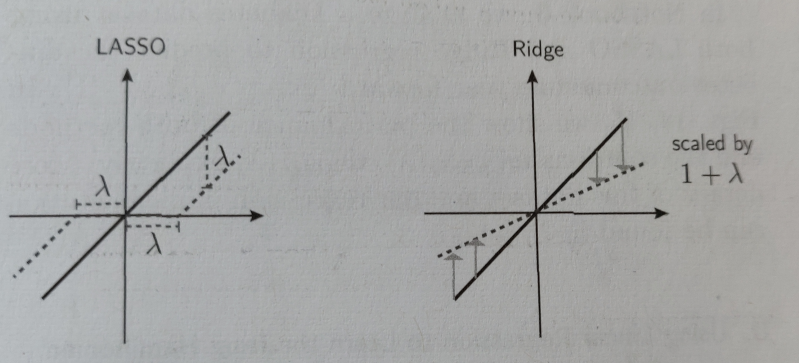
\includegraphics[width=0.7\linewidth]{gfx/LassoVsRidge}
	\caption{}
	\label{fig:lassovsridge}
\end{figure}
\begin{mybox}{On the hyperparameter}
	The regularization parameter $\lambda$ affects the weights (features) the model (LASSO, Ridge) learns on a data set.
\end{mybox}

\subsubsection{A note on LASSO and Ridge}
Note that both LASSO and Ridge regression are convex in  $\mw$ . What's more, Ridge is actually a strictly convex problem (assuming  $\lambda >0$ ) due to presence of $L_2$ penality. In fact, this is always true regardless of  $\mX$  and so the ridge regression solution is always well-defined.

In contrast, LASSO is not always strictly convex and hence by convexity theory, it need not have a unique solution. The LASSO solution is unique under general conditions, for example, when  $\mX$  has columns in general position. To mitigate this, one can define a modified problem called the elastic net such that the function we want to minimize is always strictly convex:
\bse 
\min_{\mw \in \mR^p}\norm{\mX \mw -\my}^2_2 + \lambda \norm{\mw}_1+\delta \norm{\mw}^2_2
\ese 
where  $λ,δ\geq 0$  are regularization parameters. Now aside from uniqueness of the solution, the elastic net combines some of the desirable properties (e.g. prediction) of ridge regression with the sparsity properties of the LASSO.
\subsubsection{Another note being a general comment on regularization}
Comparing the performance of OLS, LASSO and Ridge for the $1D$ Ising model via the coefficient of determination \ref{eq:errorR2} by looking at the parameter space of the hyperparameter $\lambda$, one can draw the following conclusions.\\
Choosing whether to use Ridge or LASSO regression turns out to be similar to fixing gauge degrees of freedom.
\begin{mybox}{Picking a regularization scheme}
	Different regularization schemes can lead to learning equivalent models but in different ’gauges’. Any information we have about the symmetry of the unknown model that generated the data should be reflected in the definition of the model and the choice of regularization.
\end{mybox}

\subsubsection{A general perspective on regularizers}
\begin{mybox}{On the hyperparameter}
	The \textbf{hyperparameter} $\lambda$ involved in e.g. LASSO and Ridge is usually predetermined, which means that it is not part of the regression process. Our learning performance and solution depends strongly on $\lambda$, thus it is vital to choose it properly. As discussed in \ref{subsec:priors}, one approach is to assume an \emph{uninformative prior} on the hyper-parameters, $p(\lambda)$, and average the posterior over all choices of $\lambda$ following this distribution. However, this comes with a large computational cost. Therefore, is is simpler to choose the regularization parameter through some optimization procedure.
\end{mybox}






\subsection{Bayesian formulation of linear regression}
\label{subsec:lregBayesian}
In the formal statistical treatment of regression, the goal is to estimate the \emph{conditional expectation} of the depndent variable given the value of the independent variable (sometimes called the covariate). To connect linear regression to the Bayesian framework, we use \ref{eq:bayesianFreqConnectionModel}. In combination with \ref{eq:bayesLogLikelihood}, we get
\bse 
l(\mt)=-\frac{1}{2\sigma^2} \sum_{i=1}^n(y_i-\mw^T \mx^{(i)})^2-\frac{n}{2} \log(2 \pi  \sigma^2) = -\frac{1}{2\sigma^2} \norm{\mX \mw -\my}^2_2 + const.
\ese
\begin{mybox}{} 
By comparing this with \ref{eq:lregOLSsolution}, it is clear that 
 performing least squares is the same as maximizing the log-likelihood of this model.
\end{mybox}

 \subsubsection{Regularization }
 What about adding regularization?
 \begin{mybox}{}
 The MAP estimate  \ref{eq:bayesMAPestimate} corresponds to regularized linear regression, where the choice of prior determines the type of regularization.
 \end{mybox}
The equivalence between MAP estimation with a Gaussian prior and Ridge regression is established by comparing \ref{eq:bayesMAPestimatorGaussianPrior} and Ridge regression \ref{eq:lregRidgeSol} with $\lambda \equiv \sigma^2/\tau^2$. An analogous derivation holds for LASSO \todo{todo ?}.

\subsection{Outlook from linear regression}
Linear regression can be applied to model non-linear relationships between input and response. This can be done by replacing the input $\mx$ with some non-linear function $\phi(\mx)$. Note that doing so preserves the linearity as a function of the parameters $\mw$, since the model is defined by their inner product $\phi^T(\mx) \mw$. This method is known as \emph{basis function expansion}.\footnote{Look into ML for physicists review for references.}







\section{Logistic Regression}
\label{sec:logisticRegression}
So far we have focused on learning from datasets for which there is a ’continuous’ output. However, a wide variety of problems, such as \emph{classification}, are concerned with outcomes taking the form of discrete variables (i.e. \emph{categories}).
\begin{example}
	For example, we may want to detect if there is a cat or a dog in an image.
\end{example}
We will now introduce \emph{logistic regression} which deals with binary, dichotomous outcomes (.e.g. True or False, Success or Failure,etc.).
\subsection{Mathematical set-up}
\subsubsection{Binary classification}
\label{subsubsec:classBinary}
Throughout this section, we consider the case where the dependent variables $y_i\in \Z$ are discrete and only take values from $m=0,\dots,M-1$ (which enumerate the $M$ classes). The goal is to predict output classes from the design matrix $\mX\in \mR^{n\times  p}$ made of $n$ samples, each of which bears $p$ features. The primary goal is to identify the classes to which new unseen samples belong.
\subsubsection{Multi-class classification}
\label{subsubsec:classMultiClass}
For multi-class classification, we can not only look at binary classification (in which the labels are dichotomous variables). One approach is to treat the label as a vector $\my_i\in \Z^M_2$, namely a binary string of length $M$ with only one component of $y_i$ being $1$ and the rest zero.
\begin{example}
	For example, $\my_i=(1,0,\dots,0)$ means data the sample $\mx_i$ belongs to class $1$.
\end{example}




\subsection{Classifiers}
Given $\mx_i$, the classifier returns the probability of being in category $m$. The following perceptron is an example of \emph{hard} classification, each datapoint is assigned to a category (i.e. $y_i=0$ or $y_i=1$). A \emph{soft} classifier on the other hand gives the probability of a given category as an output.\\
The classifiers do this by using threshold functions, which are discussed in the following \ref{subsubsec:thresholdfct}.\\
In many cases, it is favourable to work with a soft classifier.
\subsubsection{On threshold function functions}
\label{subsubsec:thresholdfct}
	A threshold function is a function that maps its input $\mx$ (a real-valued vector) to an output value $f(x)$ (a single binary value).
One simple way to get a discrete output is to have sign (or threshold) functions that map the output of a linear regressor to $\{0,1\}$. The following are possible:
\begin{enumerate}
	\item The \emph{sign} function 
\be
\label{eq:logRegsign}
\sigma(s_i)=\text{sign}(s_i)= \left\{\begin{array}{ll}
	1 & \text{if } s_i\geq 0 \\
	0 & \text{otherwise} \\
\end{array}  \right\}
\ee
is employed for hard classification.
\item The \emph{logistic} (or \emph{sigmoid}) function
\be 
\label{eq:logRegSigmoid}
\sigma(s) = \frac{1}{1+e^{-s}}, \quad 1-\sigma(s) = \sigma(-s).
\ee 
\end{enumerate} 
\subsection{Perceptron - a motivation}
Before delving into the details of logistic regression, it is helpful to consider a slightly simpler classifier.
\begin{mybox}{Perceptron}
	Consider a linear classifier that categorizes examples using a weighted linear-combination of the features and an additive offset:
	\be 
	\label{eq:logRegPerceptron}
	s_i = \mx^T_i \mw + b_0  \equiv \mathbf{\mathbb{x}}^T_i \mathbf{\mathbb{w}},
	\ee 
	where we use the short-hand notation $\mathbf{\mathbb{x}}_i=(1,\mx_i)$ and $\mathbf{\mathbb{w}}=(b_0,\mw)$. This function takes values on the entire real axis. IN the case of logistic regression, however, the labels $y_i$ are discrete variables. Using the sign function \ref{eq:logRegsign} to create discrete outputs via hard classification, we obtain the \emph{perceptron} model.\\
	In the modern sense, the perceptron is an algorithm for learning a binary classifier called a  \emph{threshold function}, see \ref{subsubsec:thresholdfct}.
\end{mybox}















\subsection{Definition of logistic regression - Bayesian}
This is a binary classification problem, see \ref{subsubsec:classBinary}.
Here we define logistic regression and discuss the minimization of its corresponding cost function (the \emph{cross entropy}). 
\begin{mybox}{Logistic regression}
	Logistic regression is the canonical example of a soft classifier. In logistic regression, the probability that a data point $\mx_i$ belongs to a category $y_i = \{0,1\}$ is given by 
	\begin{align*}
		P(y_i=1|\mx_i,\mt)&= \frac{1}{1+e^{-\mathbf{\mathbb{x}}^T_i \mt}} = \sigma(\mathbf{\mathbb{x}}^T_i \mathbf{\mathbb{w}})\\
		P(y_i=0|\mx_i,\mt) &= 1-P(y_i=1|\mx_i,\mt)
	\end{align*}
	where $\mt = \mathbf{\mathbb{w}}$ are the weights we wish to learn from the data. The cost function of logistic regression, the \emph{cross entropy}, is found to be
	\be 
	\label{eq:logregCrossEntropy}
	\mC(\mathbf{\mathbb{w}} )= \sum_{i=1}^n \left[-y_i \log \sigma(\mathbf{\mathbb{x}}^T_i \mathbf{\mathbb{w}}) -(1-y_i) \log\left(1-\sigma(\mathbf{\mathbb{x}}^T_i \mathbf{\mathbb{w}})\right)\right].
	\ee 
	In practice, we usually implement the cross-entropy (like in linear regression) with additional regularization terms, usually $L_1$ and $L_2$ regularization.
\end{mybox}
\begin{mybox}{Minimizing the cross entropy}
	The cross entropy is a convex function of the weights $\mathbb{w}$ and, therefore, any local minimizer is a global minimizer. Minimizing this cost function leads to 
	\be 
	\label{eq:logregCrossEntropyMinimized}
	0 = \mathbf{\nabla} \mC(\mathbb{w}) = \sum_{i=1}^n \left[\sigma(\mathbb{x}^T_i \mathbb{w}) - y_i\right]\mathbb{x}_i.
	\ee 
	In words, the gradient points in the sum of training example directions weighted by the difference between the true label and the probability of predicting that label.
	Equation \ref{eq:logregCrossEntropyMinimized} defines a transcendental equation for $\mathbb{w}$, the solution of which, unlike linear regression, cannot be written in a closed form. For this reason, one must use numerical methods such as \ref{sec:gd} to solve this optimization problem.
\end{mybox}\footnote{However, as a word of caution, note there is a generic instability in the MLE procedure for linearly separable data)}
In the notebooks, one looks at two examples to train a logistic regressor to classify binary data.
We call \emph{one-hot} a group of bits where only one bit is $1$ and all others $0$, i.e. representing states: $\ket{1}=(1,0,\dots,0), \ket{2}=(0,1,0,\dots,0)$.
\subsubsection{On the 2d Ising example}
Given an Ising state, we would like to classify whether it belongs to the ordered or the disordered phase, without any additional information other than the spin configuration itself. This categorical ML problem is well suited for logistic regression, and will thus consist of recognizing whether a given state is ordered by looking at its bit configurations. Notice that, for the purposes of logistic regression, the $2D$ spin state of the Ising model will be flattened out to a $1D$ array, so it will not be possible to learn information about the structure of the contiguous ordered $2D$ domains. SUch information can be incorporated using deep convolutional neural networks.\\
We use both ordered and disordered states to train the logistic regressor and, once the supervised training procedure is complete, we will evaluate the performance of our classification model on unseen ordered, disordered, and near-critical states. Here, we deploy the \emph{liblinear} routine (the default for Scikit' s logistic regression) and stochastic gradient descent to optimize the logistic regression cost function with $L_2$ regularization. We define the accuracy of the classifier as the percentage of correctly classified data points. Comparing the accuracy on the training and test data, we can study the degree of overfitting.\\
Similar to the linear regression examples, we find that there exists a sweet spot for the SGD regularization strength $\lambda$ that results in optimal performance of the logistic regressor.
\subsubsection{SUSY }
Here we will use logistic regression in an attempt to find the relative probability that an event is from a signal or a background. Is a good classification problem with noisy data, how to discriminate against the background ? Some signal events look background-like, and some background events look signal-like to our discriminator.
\subsection{SoftMax regression}
In this section we generalize logistic regression to the case of multiple categories which is called \emph{SoftMax regression}. This is a multi-class classification problem \ref{subsubsec:classMultiClass}.
\begin{mybox}{SoftMax regression}
	The probability of $\mx_i$ being in class $m^\prime$ is given by
	\be
	\label{eq:logregSoftMaxfct} 
	P(y_{im^\prime} =1 | \mx_i,\{\mathbb{w}_k\}^{M-1}_{k=0})=\frac{e^{-\mathbb{x}^T_i \mathbb{w}_{m^\prime}}}{\sum_{m=0}^{M-1} e^{-\mathbb{x}^T_i \mathbb{w}_m}},
	\ee 
	where $y_{im^\prime} \equiv [\my_i]_{m^\prime}$ refers to the $m^\prime$-th component of vector $\my_i$. This is known as the \emph{SoftMax} function. The generalized cost function reads
	\begin{align}
	\label{eq:logregSoftMaxcostFct}
	\mC(\mathbb{w}) &= - \sum_{i=1}^n \sum_{m=0}^{M-1} \left[ y_{im} \log P(y_{im}=1|\mx_i, \mathbb{w}_m) \right.. \\
	&\left. + (1-y_{im }) \log\left(1-P(y_{im} =1 |\mx_i ,\mathbb{w}_m)\right)\right],
	\end{align} 
	which reduces to the cross entropy \ref{eq:logregCrossEntropy} for $M=1$, i.e. for only two possible classes.
\end{mybox}




\section{Ensemble Methods - On combining models}
\label{sec:ensembles}
\subsection{Introduction}
Ensemble methods combine predictions from multiple, often weak, statistical models to improve predictive performance. Ensemble methods, such as random forests, and boosted gradient trees, such as XGBoost, undergird many of the winning entries in data science competitions such as Kaggle, especially on structured datasets. Note that Neural Networks generally perform better than ensemble methods on unstructured data, images and audio. Even in the context of NN, it is common to combine predictions from multiple neural networks to increase performance on tough image classification tasks.
\subsubsection{Motivation}
We will give an overview of ensemble methods and provide rules of thumb for when and why they work.\\
On one hand, the idea of training multiple models and then using a weighted sum of the predictions of all these models is very natural. On the other hand, one can also imagine that the ensemble predictions can be much worse than the predictions from each of the individual models that constitute the ensemble, especially when pooling reinforces weak but correlated deficiencies in each of the individual predictors. Thus, it is important to understand when we expect ensemble methods to work.\\
As we saw in \ref{subsubsec:biasvarianceMathematicalEnsemble}, the key to determining when ensemble methods work is the degree of correlation between the models in the ensemble.
\subsubsection{Benefits of Ensemble Methods before diving in}
Three distinct shortcomings that are fixed by ensemble methods are: statistical, computational, and representational.\\
The first reason is statistical. When the learning set is too small, a learning algorithm can typically find several models in the hypothesis space $\mH$ that all give the same performance on the training data. Provided their predictions are uncorrelated, averaging several models reduces the risk of choosing the wrong hypothesis. The second reason is computational. Many learning algorithms rely on some greedy assumption or local search that may get stuck in local optima. As such, an ensemble made of individual models built from many different starting points may provide a better approximation of the true unknown function than any of the single models. Finally, the third reason is representational. In most cases, for a learning set of finite size, the true function cannot be represented ba any of the candidate models in $\mH$. By combining several models in an ensemble, it may be possible to expand the space of representable functions and to better model the true function.\\
\\ 
The increase in representational power of ensembles comes from the fact that it is more advantageous to combine a group of simple hypotheses than to utilize a single arbitrary linear classifier. This of course comes with the price of introducing more parameters to our learning procedure. But if the problem itself can never be learned through a simple hypothesis, then there is no reason to avoid applying a more complex model. Since ensemble methods reduce the variance and are often easier to train than a single complex model, they are a powerful way of increasing representational power (also called expressivity in the ML literature).\\
\\
How should we construct ensembles ?\\
\begin{enumerate}
	\item Try to randomize ensemble construction as much as possible to reduce the correlations between predictors in the ensemble. This ensures that our variance will be reduced while minimizing an increase in bias due to correlated errors.
	\item The ensembles will work best for procedures where the error of the predictor is dominated by the variance and not the bias. Thus, these methods are especially well suited for unstable procedures whose results are sensitive o small changes in the training dataset.
	\item Although the discussion above was derived in the context of continuous predictors such as regression, the basic intuition behind ensembles applies equally well to classification tasks. Using an ensemble allows one to reduce the variance by averaging the result of many independent classifiers. As with regression, this procedure works best for unstable predictors for which error are dominated by variance due to finite sampling rather than bias.
\end{enumerate}



\subsection{Bagging}
\label{subsec:ensemblesBagging}
\subsubsection{Bootstrapping}
\subsection{Random Forests}
\label{subsec:ensemblesRandomForest}
\subsection{Gradient Boosted Trees and XGBoost}
\label{subsec:ensemblesGBoostedTreesandXGBoost}
\subsection{Different methods}
Bagging, boosting, random forests, and gradient boosted trees such as XGBoost.
\subsubsection{Bagging}












\section{In Introduction to Feed-Forward Deep Neural Networks (DNNS)}
\label{sec:dnn}


\chapter{Ideas for problems to work on}
\section{Physics problems}
\subsection{Cosmology}
\begin{enumerate}
	\item Maybe write a classification logistic regressor, or deep CNN to classify where dark matter halos have their boundary. It is very difficult to define a boundary of such a spread out object with confidence, maybe find criteria via classification ML technique ?
\end{enumerate}
\subsection{QFT}